\section{Web bányászat}

Web bányászat, vagy angol kifejezésben Web mining, alatt azt a folyamatot értjük, amely által új, eddig nem ismert, de hasznos információt fedezünk fel az Interneten található adatok között. Mindezt a cégek arra használják, hogy új értékes információkat gyűjtsenek, ezeket feldolgozzák, majd ezek által a felhasználókat vagy fogyasztókat jobban megismerjék. Ez a folyamat az úgynevezett adat bányászat technikát alkalmazza ahhoz, hogy automatikusan kinyerje az adatokat az Internetről \cite{gorunescu2011data}. 

Számos más technikát is alkalmaztak már új információk kinyerésére, az így is hatalmas és egyre növekvő adat mennyiségből, mint például az Information retrieval, Information extraction illetve gépi tanulás. Az Information retrival működési elve az, hogy a szöveg indexelésé után nyeri ki a hasznos információt. Az Information Extraction arra fokuszál, hogy csak a lényeges információt nyerje ki, míg az előbb említett inkább hasznos dokumentumokat jelöl meg. A gépi tanulásos módszer nem kötődik direkt módon a Web Scraping-el viszont segítséget nyújt a szövegek osztályozási folyamatában. A web bányászatot három fő kategóriába soroljuk, ahogy az látható az \ref{fig:web_mining_rendszertana} ábrán is.

\begin{figure}[h]
    \centering
    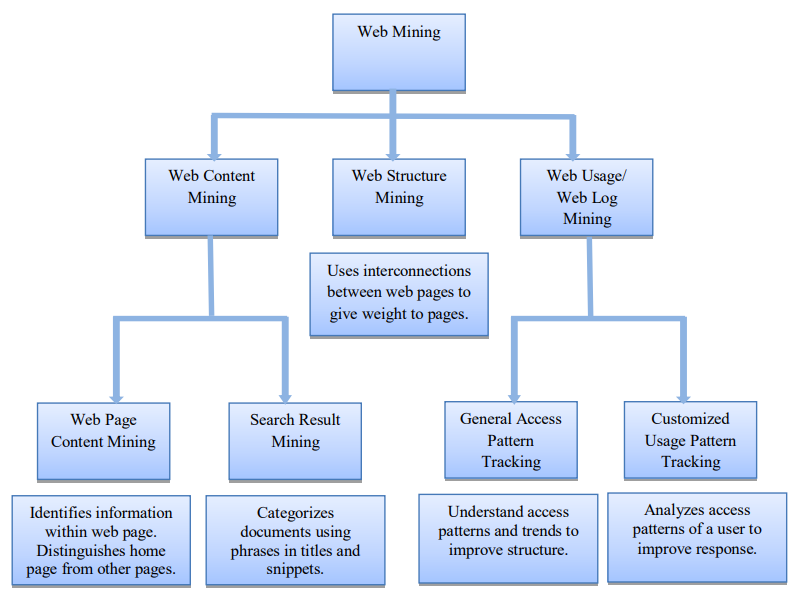
\includegraphics[scale=1, width=\textwidth]{figures/images/web_mining_rendszertan.png}
    \caption{A Web Bányászat rendszertana \cite{johnson2012web}}
    \label{fig:web_mining_rendszertana}
\end{figure}

A Web Content Mining vagy magyarul webes tartalom bányászat, olyan tartalmakra fekteti a hangsúlyt, mint például szöveg, kép, audió, video, metaadatok, hiperlinkek. Ezek tanulmányozása, segít nekünk megérteni a felhasználók, vásárlók viselkedését mely által a weboldalak teljesítményét növelni lehet a későbbiekben, hogy azok jobban, illetve hatékonyabban működjenek. 

Mivel a webes tartalom bányászat megvizsgálja úgy a kereséseket, mint azoknak a konkrét tartalmát ezért ezt is tovább lehet osztani két kategóriába, Keresési Eredmény, illetve Weboldal Tartalom bányászat. Nevükből adódóan, ezek kiegészítik egymást, mivel a tartalom bányászat azon oldalakon történik, melyeket korábban megvizsgált és ígéretesnek talált a Keresési eredmény általi elemzés. A Web Structure Mining egy olyan ágazat, mely struktúrák bányászásával foglalkozik, mint például HTML vagy XML címkék, amely által weboldalak közötti kapcsolatot tud felismerni, ezáltal súlyokat rendelve azokhoz. A Web Usage Mining által lehet megérteni a különböző használati mintákat, amelyeket a felhasználók követnek, ezeket főként naplózás, felhasználók profiljai, sütik, könyvjelzők által, de ugyanide tartoznak a különböző egér mozdulatok vagy görgetési adatok is.

\section{Web Struktúra Bányászat}

Rengeteg új adat generálódik az Interneten, napról napra az adat mennyiség exponenciálisán növekszik. Bőségesen állnak rendelkezésünkre szolgáltatások, illetve információk, elektronikus áruházak, elektronikus újságok, közösségi oldalak formájában, hogy csak párat említsünk. Habár ezen adatok fogyasztás céljára lettek szánva, sok időt el lehet tölteni az adatok kinyerésével és elemzésével. Továbbá, a weboldalak adatai HTML, illetve más webre szánt formátumban vannak jelen, amely megnehezíti az automata feldolgozást. Ez lett a mozgató rugója az ezen a téren zajló kutatásnak, mint például a Web Scraping.

A Web Structure Mining, vagy ismertebb nevén Web Scraping, az a folyamat, amely által hasznos információkat nyerünk ki egy weboldal HTML kódjából, amely az Internet fő formázási eszköze \cite{dastidar2016intelligent}. Az egyik metodológia megállapította, a rendezett annotációk, melyek nem mások, mint gépek számára is értelmezhető leíró információk az adott oldalra tekintve, egy külön szemantikus rétegben vannak tárolva, elválasztva a weboldaltól, ezáltal megkönnyítve és felgyorsítva a bányászási folyamatot, mivel először ezeket a fontos metaadatokat dolgozza fel, majd csak ezt követően magát a weboldalt.

A HTML struktúráját tekintve, két fő adat típust lehet bányászni belőle. Az egyik a felhasználó által generált - a másik pedig a metaadat. A felhasználó által generált adat bármi olyan típusú adatra vonatkozik, amelyet a felhasználó hozott létre vagy adott hozzá a weboldalhoz, akár személyesen akár egy közösségi platform hozzácsatolásával. A metaadat definíció szerint olyan adat, amely leír egy másik adatot \cite{landers2016primer}, ezek általában minden weboldalon megtalálhatók, fontosabb leíró adatokat tartalmazva, mint például szerző, cím, cikkek eseten megjelenés időpontja, kulcsszavak. Ezek általában nem láthatóak a felhasználó számára, viszont kiolvashatóak az adott oldal HTML kódjából \cite{landers2016primer}.

\subsection{Szemelyre szabott információ lekérése példával illusztrálva}

Tegyük fel, hogy egy személy fárasztónak találja, hogy a nap végen a fontos vagy számára értékes hírek után keressen, vagy előkeresse a kedvenc sport csapata elért eredményeit. Egy intelligens Web Scraper a tökéletes eszköz ebben az esetben, mivel az időközönként végig tudja böngészni az Internetet a felhasználó által megszabott témakörökben található információk után kutatva, vagy akár specifikus kulcsszavakat tartalmazó híreket előkertivé. Ez egy előre weboldalakat tartalmazó listán menne végig, melyet a felhasználó határoz meg, hogy a számára hiteles információt kapja meg \cite{dastidar2016intelligent}.

Egy másik példa egy Web Scraper felhasználására az, amikor például egy vásárló több terméket is kinézett magának, több különböző weboldalon. Ha esetleg nem szeretné azonnal megvásárolni a terméket, hanem csak követni annak árát, akkor esettől függően, több oldalra is be kell jelentkeznie, több felhasználóval oldalankent, de legjobb esetben is számos oldalt kellene naponta megfigyeljen és lejegyezzen. Egy Web Scraper abban könnyítené meg a felhasználó dolgát, hogy például egy böngészős kiegészítő keretein belül, a vásárló hozzá tudja adni egy listához a terméket és attól a pillanattól, a program naponta akár többször is le tudja kérni a termék árát, anélkül, hogy a felhasználó bármit is tenne. Ezáltal egy helyen lenne a vásárló több terméke, és pár kattintással tisztább kepét alkothat a termékek árára vonatkozóan

\section{A Web Scraping gyakori alkalmazásai}

\begin{itemize}
    \item Online ár összehasonlítás – ugyanazon termék arának összehasonlítása több weboldalon, pl. https://www.compari.ro/, https://www.price.ro/ 
	\item Contact Scraping – általában email címeket gyűjtenek, marketing céljából
    \item Időjárással kapcsolatos adatok gyűjtése
    \item Weboldal változásainak figyelése
	\item Több forrásból származó adat egyesítése
	\item Kedvezmeny kuponok pl. pouch – chrome extension
	\item Álláshirdetések összesítése
	\item Brand monitoring – egy bizonyos márkához tartozó adatokat gyűjtik, általában az ahhoz társított véleményre kíváncsiak
    \item Piac tanulmány – Egy adott termék piacon való elhelyezkedését, illetve potenciális sikerességet próbáljak megjósolni a bányászott adatok átvizsgálásával.
\end{itemize}

\section{Web Scraping Technikák}

Számos technika áll rendelkezésünkre melyekkel az adatgyűjtést végezhetjük, ezeket mindig az adott helyzetnek megfelelően kell kiválasztani, főként a hatékonyságot tartva szemelőt. Ebben a részben a Web Scraping egy pár technikája kerül röviden ismertetésre.

Copy-paste - Időközönként valaki kézzel történő adatgyűjtést, valamint vizsgálatot végez. Adott helyzetekben ez a leghatékonyabb módszer, viszont nagyon hajlamos a hibákra, sok időt és fáradságot vesz igénybe az ember részéről, amíg a nagy adathalmazokat feldolgozza.

Reguláris kifejezések - Ez egy egyszerű és erőteljes megközelítése az információ gyűjtésnek. A UNIX vagy más programozási nyelv által használt reguláris kifejezés illesztésen alapszik.

HTML Parsing – Félig strukturált lekérdező nyelvek segítségével elemezni, illetve módosítani a weboldalak tartalmát.

DOM Parsing – A böngészőkbe beépített kezelő programok segítségével, az erre a célra fejlesztett alkalmazások lekérhetik a kliens oldalon dinamikusan létrejött tartalmakat is, mellyel utána fel tudják építeni a DOM fát, ebben pedig könnyebben lehet specifikus adatok után keresni.

Web Scraping Szoftver – Számos szoftver áll rendelkezésünkre, amelyeket személyre szabott keresésre lehet használni. 

Mesterséges Intelligencia – Több helyen is kísérleteznek gépi tanulásos adatbányászattal, melynek az a célja, hogy a gépek megtanulják úgy értelmezni a weboldalakat, ahogy azt az emberek tennék.

\section{Web Scraping Szoftverek}

A Web Scraping szoftverek rendkívül fontos szerepet játszanak ezen a téren, mivel automatizálják és rendkívül felgyorsítják az adat-gyűjtő, valamint feldolgozó folyamatot. Számos ilyen szoftver található a piacon, a maga előnyeivel és hátrányaival. Ezeknek az ára a funkcionalitásuk függvényében, valamint a támogatás és frissítési időszakok függvényében változik. 

Visual Web Ripper\footnote{\url{http://visualwebripper.com/}} – Az egyik legfejletteb web scraping szoftver, melyet a Sequentum csoport fejlesztett 2006-tól kezdődően. Weboldalakról gyűjtött információk bányászására használják, úgy egyszerű weboldalak, mint e-commerce oldalak esetében, mint például eBay, Amazon, magento, azonban titkosított tartalmak eseteben is segítségünkre lehet. A bányászott adatokat kimenthetjük adatbázisba vagy CSV, illetve XML formátumban is. Előnye, hogy vizuális felülettel rendelkezik, ezért rendkívül egyszerűen ki lehet választani, hogy pontosan mit is szeretnénk. Egyszeri fizetéssel lehet megvásárolni a szoftvert, \$349.00 áron\footnote{\label{price_disclaimer}Az árak aktualitásáért lásd a szolgáltató weboldalát}, viszont fontos szempont, hogy ezen alkalmazás elveszti a gyártó általi támogatottságát 2021-gyel kezdődően, kivételt kepézve azon esetek, ahol a vásárlóval karbantartási szerződés van érvényben, mely túlhaladja ezt az időpontot.

Web Content Extractor\footnote{\url{https://www.webcontentextractor.com/}} – Nagyon jó automatizálási lehetőséget nyújt, rendkívül egyszerűen használható, pár kattintással meg lehet adni a kivánt mintát, ami szerint majd adatokat fog gyűjteni. A program rugalmas, abból a szempontból, hogy nem próbálja túlokoskodni a felhasználót, hanem egy előlnézetet ad az eredményről, majd a felhasználó maga végezheti el a szükséges módosításokat, amennyiben szükség van erre. Ezt a szoftvert, bérlet alapú előfizetéssel lehet megszerezni, több változat is elérhető, az árak \$30 - \$150 / hónap\footref{price_disclaimer} között mozognak.

Mozenda\footnote{\url{https://www.mozenda.com/}} – Az egyik legegyszerűbben használható szoftver ezen a téren, ami lehetővé teszi a kevésbé technikailag hozzáértő személyeknek is, az egyszerű bányászásokat. Fő különbsége más alkalmazásokhoz kepést, hogy maga az adatbányászati folyamat a felhőben történik és nem a felhasználó erőforrásait felhasználva, amely hatalmas előnyt jelenthet. Elérhető egy 30 napos próba csomag is, ami után \$250/hónap-tól\footref{price_disclaimer} kezdődően változnak az árak, a választott csomag függvényében.

Screen-Scraper\footnote{\url{https://www.screen-scraper.com/}} – Nagyon fejlett web scraping alkalmazás, amelyet több változatban is el lehet érni. Az alapszínűt verzió ingyenes, ezzel egyszerűbb adatok után lehet bányászni, könnyen kezelhető, nem kell sok technikai tudás hozzá. Más változatok, mint például a profi vagy vállalkozás szintű verziók már sokkal komplexebbek, több lehetőséget nyújtanak. Nagy előnyé, hogy más rendszerekkel könnyen összeférhető pl. Java, ezért fel lehet használni más, nagyobb szintű programokban is.

% \usepackage[symbol]{footmisc}
% \renewcommand{\thefootnote}{\fnsymbol{footnote}}
% \footnote[aster]{}

Természetesen sok más program is rendelkezésünkre áll, melyek hasonló funkcionalitásokkal rendelkeznek, minden esetben az adott alkalmazásnak megfelelőt és legjobban illőt érdemes választani a nagyobb hatékonyság érdekében. Egyéb web scraper szoftverek \cite{sirisuriya2015comparative}: WebHarvy, Easy Web Extract, WebSunDew, FMiner, Scrapy, import io. 

% \let\thefootnote\relax\footnote{* Az árak aktualitásáért lásd a szolgáltató weboldalát}
% \renewcommand{\thefootnote}{\alph{footnote}}
% \footnotetext{* Az árak aktualitásáért lásd a szolgáltató weboldalát}

\section{Legális és Etikai keretek}

Ebben a fejezetben a legális valamit etikai kérdésekről lesz szó, amely elég megosztó, illetve nem teljesen egyértelmű terület. Egyenesen a Web Scraping-et nem szabályozza semmilyen törvény, de több területen is problémába lehet ütközni, ilyen például a védett tartalom, az úgynevezett szerződésszegés vagy GDPR. Attól függően, hogy a bányászat milyen országhoz tartozó területen zajlik, figyelembe kell venni az ottani törvénykezést is, ezért is nehéz konkrétan jellemezni legalitási szempontból. A legpontosabb jellemzés talán az lenne, hogy van, ami igen és van, ami nem.

\subsection{Felhasználói feltételek}

Ugyanúgy, mint egy szoftver vagy szolgáltatás esetén, amikor egy weboldalt használunk el kell fogadnunk bizonyos felhasználói feltételeket, melyek leggyakrabban kis felrúgó ablakkent jelennek meg, amikor először látogatunk a weboldalra, vagy ezeket a regisztrálás folyamán tudatosítják velünk. Amennyiben valamilyen módon megszegjük ezeket a feltételeket, érvénybe lép a fentebb említett szerződésszegés. Mivel ez csak akkor érvényes, ha a felhasználó explicit elfogadja a feltételeket, jogi szempontból nem nehéz kizárni a Web Scrapinget. 

\subsection{Szerzői jogok}

Bányászni vagy újra publikálni olyan adatokat vagy információkat, amelyeknek a szerzője explicit módon fenntartja a szerzői jogokat, legális szempontból szerzői jogsértésnek minősül. Ugyanakkor egy weboldal nem minden esetben rendelkezik a felhasználói által generált adatokkal, vegyünk példának egy film értékelő oldalt, ahol a felhasználók kifejtik a véleményüket \cite{krotov2018legality}. Más ebbe a kategóriába tartozó tartalmak például a videók, kepék, zenék, adatbázisok, cikkek. Maga a bányászása ezeknek az adattoknak nem teszi illegálissá, a felhasználási módjuk határozza meg azt, hogy milyen kategóriába soroljuk azt. 

\subsection{GDPR}

Az Európai Unió által érvénybe léptetett Általános Adatvédelmi Rendelet\footnote{\url{https://gdpr-info.eu/}} alapján nem tiltott az adatbányászat, kivételt kepézve, ha ez a tevekénység nem tartalmaz személyes adatokat. Ilyennek minősül a név, lakcím, email cím, telefonszám, bankkártya adatok, banki adatok, IP cím, születési dátum, foglalkoztatási információk, orvosi adatok, személyes fotók vagy videók.

\subsection{Weboldal Károsítása}

Ha bármilyen tevekénység által, amelyet a Web Scraper végez, túlterheljük az adott weboldal szervereit vagy bármilyen módon sértjük, gátoljuk annak működését bűncselekménynek számít és legális következményei lehetnek. Ehhez azonban a kárnak anyaginak kell lennie, valamint könnyen bizonyíthatónak bíróság elött, ahhoz, hogy bármiféle kártérítési kérelemre legyen jogosult a weboldal \cite{krotov2018legality}. 

A fentieket figyelembe véve tehát, nem lehet egyértelmű választ adni arra, hogy a Web Scraping legális-e vagy sem. Helyette a válasz az, hogy helyzettől függ. Maga a Web Scraping nem illegális, viszont akár az is lehet a következő három dolog függvényében \cite{isWSLegal}. 

\begin{itemize}
    \item Hogyan lett bányászva az adat?
    \item A bányászott adat típusa
    \item Hogyan lesz felhasználva a bányászott adat?
\end{itemize}

Ahhoz, hogy eldöntsük az esetünk legalitását meg kell vizsgálni, hogy az adat, amit szeretnénk bányászni publikusan elérhető-e vagy sem. Ha az adat eléréséhez nem szükséges bejelentkezni egy adott oldalra akkor a felhasználói feltételek nem érvényesek ezért legálisan lehet bányászni, mivel ez az adat publikusnak számít. Ha bejelentkezésre van szükség a bányászni kívánt adat eléréséhez, akkor a felhasználói feltételek tanulmányozásával el kell dönteni, hogy legális-e vagy sem, mivel azok elfogadásával legálisan alkalmazhatóvá vált számunkra, azaz a megszegésük jogi következményeket vonhat maga után.

A bányászott adat típusa szerint két formájára kell nagyon odafigyelni, Személyes Adatok és Szerzői Jogokkal rendelkező adatok, ezek fentebb részletesebben is tárgyalva voltak.

Az adatok felhasználása során figyelembe kell venni, hogy az illegális módon vagy csalás által történő adatgyűjtést minden állam bünteti, tehát ez bűncselekménynek minősül. Amennyiben olyan tartalmakat bányászunk melyek bizalmas vagy bármi féle módon védett információt tartalmaznak, ezeknek felhasználása ugyancsak törvényszegést jelent és az erényben levő büntető eljárások érvényesek. Természetesen, legtöbb esetben már maga az törvénysértő lehet, hogy ezekhez az adatokhoz jogosultság nélkül fértünk hozzá, ezért egyértelműen nem felhasználhatóak ezek az adatok. 

Leegyszerűsítve, három alapvető kérdésre kell választ adni, ahhoz, hogy eldöntsük legális-e az adat bányászat, amelyet végre szeretnénk hajtani: 

\begin{itemize}
    \item Bejelentkezés által elérhető adatot bányászok?
    \item Személyes adatot bányászok?
    \item Szerzői jogokkal rendelkező adatot bányászok?
\end{itemize}

Amennyiben mindhárom kérdésre nemleges a válasz, legálisnak bizonyul adott esetben a Web Scraping. Azonban, ha bármelyik kérdésre pozitív választ adunk nagy valószínűséggel újra kell gondolni és figyelmesebben megvizsgálni az eset legális mivoltát. Ugyanakkor egyik esetben sem szabad megfeledkezni arról, hogy minden ország másképp kezelheti ezen kérdéseket, ezért ilyen értelemben is vizsgálódnunk kell.